%  !TeX  root  =  user_guide.tex 
% % \section{Using external QGIS Python Plugins}\label{sec:external_plugins}\index{plugins}
\section{Utiliser des extensions externes en Python pour QGIS}\label{sec:external_plugins}\index{extensions}

% when the revision of a section has been finalized, 
% comment out the following line:
% \updatedisclaimer

%External QGIS plugins are written in Python. They are stored in either 
%the 'Official' or 'User contributed' QGIS Repostories, or in various other external 
%repositories maintained by individual authors. 
%Table \ref{tab:external_plugins} shows a list of curently available 'Official' 
%plugins, with a short description.
%Detailed documentation about the usage, minimum QGIS version, homepage, authors, 
%and other important information are provided with the external plugins themselves 
%and is not included in this manual.
%\footnote{Updates of core plugins may be 
%available in this repository as external overlays.} 
%\footnote{fTools, Mapserver Export, and the Plugin Installer are Python plugins, 
%but they are also part of the QGIS sources, and are automatically loaded and enabled inside
%the QGIS Plugin Manager (see Section~\ref{sec:load_external_plugin}).}

Les extensions QGIS externes sont écrites en python. Elles sont stockées dans un dépôt officiel ou dans des dépôts de contribution d'utilisateurs ou dans des dépôts externes maintenus par des auteurs individuels. Le tableau~\ref{tab:external_plugins} montre une liste d'extensions officielles actuellement disponibles avec une courte description. La documentation détaillée sur l'utilisation, la version minimale requise de QGIS, l'auteur et d'autres informations d'importance sont fournies par les extensions externes et ne sont pas couvertes dans ce manuel.\footnote{Les mises à jour des extensions principales peuvent également être disponibles via ce dépôt} \footnote{L'installateur d'extensions python est également une extension python externe, mais il fait partie des sources de QGIS et est donc automatiquement chargé et sélectionné dans le gestionnaire d'extension de QGIS (voir la section~\ref{sec:load_external_plugin}).}

%You will find an up-to-date list of 'Official' plugins in the Official QGIS 
%Repository at \url{http://qgis.osgeo.org/download/plugins.html}. This list is also available 
%automatically from the \filename{Plugins installer} via \dropmenuopttwo{plugin_installer}{Fetch Python
%Plugins...}.
Vous trouverez une liste à jour des extensions présentes dans le dépôt officiel de QGIS à \url{http://qgis.osgeo.org/download/plugins.html}. Cette liste est disponible automatiquement depuis la fenêtre \filename{Installateur d'extensions Python} de \\ \dropmenuopttwo{plugin_installer}{Récupérer les extensions pythons...}.

%\begin{table}[H]
%\centering
%\caption{Current moderated external QGIS Plugins}\label{tab:external_plugins}\medskip
%\small
% \begin{tabular}{|l|l|p{4in}|}
%\hline \textbf{Icon} & \textbf{External plugin} & \textbf{Description}\\
%\hline
%
\includegraphics[width=0.7cm]{zoom2point_icon}
% & Zoom To Point \index{plugins!Zoom To Point} & Zooms to a coordinate 
%  specified in the input dialog. You can specify the zoom level as well to 
%  control the view extent.\\
%\hline
%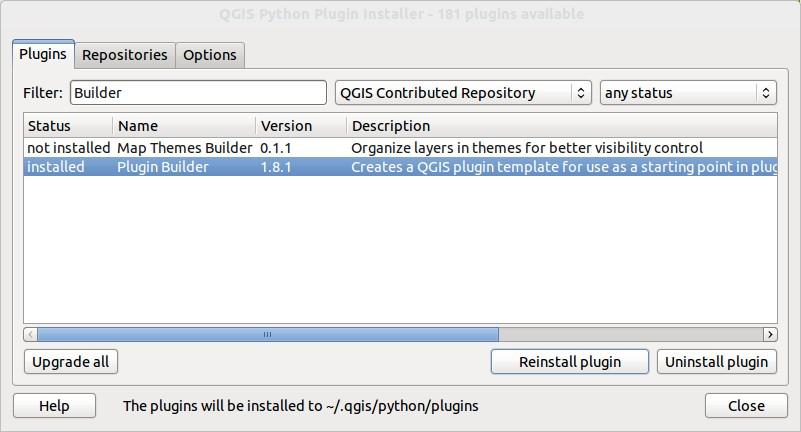
\includegraphics[width=0.7cm]{plugin_installer}
% & Plugin Installer \index{plugins!Plugin Installer} & The most recent Python Plugin Installer.\\
%\hline
\begin{table}[H]
\centering
 \begin{tabular}{|l|l|p{8cm}|}
\hline \textbf{Icône} & \textbf{Extension externe} & \textbf{Description}\\
\hline

\includegraphics[width=0.7cm]{zoom2point_icon} & Zoom vers un point \index{extensions!Zoom vers un point} & Zooms vers des coordonnées définies dans la boîte de dialogue. Vous pouvez définir également le niveau de zoom pour contrôler l'étendue de la vue.\\
\hline
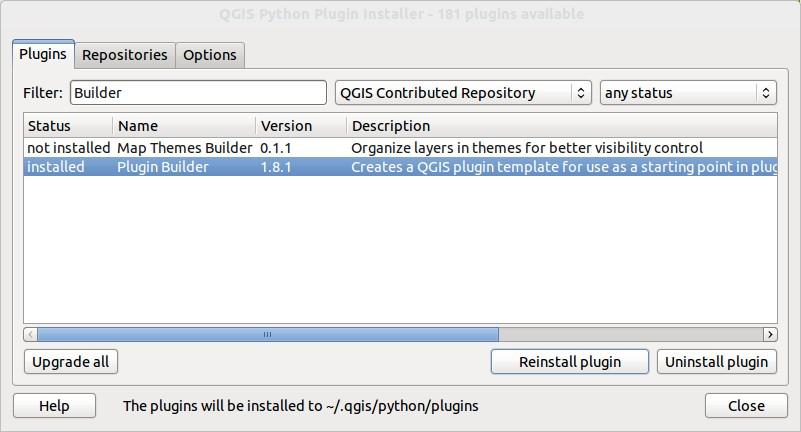
\includegraphics[width=0.7cm]{plugin_installer} & Installateur d'extensions Python \index{extensions!Installateur d'extensions}&\\
\hline
\end{tabular}
\caption{Extensions QGIS externe actuellement modéré}\label{tab:external_plugins}
\end{table}

%A detailed description of the installation procedure for external python plugins can be found in 
%Section \ref{sec:load_external_plugin}.
Une description détaillée de l'installation pour les extensions python externes peut être trouvée dans la section \ref{sec:load_external_plugin}.

%\begin{Tip} \caption{\textsc{Add more repositories}}
%\qgistip{To add the 'User contributed' repository and/or several external author repositories, open the 
%Plugin Installer (\mainmenuopt{Plugins} > \dropmenuopttwo{plugin_installer}{Fetch Python Plugins...}),
%go to the \tab{Repositories} tab, and click \button{Add 3rd party repositories}. 
%If you do not want one or more of the added repositories, they can be disabled via the 
%\button{Edit...} button, or completely removed with the \button{Delete} button.
%}
%\end{Tip}

\begin{Tip} \caption{\textsc{Ajout d'autres dépôts}}
Pour ajouter le dépôt des contributions d'utilisateurs ou des dépôts externes, ouvrez l'installateur d'extensions (\mainmenuopt{Extensions} > \dropmenuopttwo{plugin_installer}{Récupérer les extensions pythons...}), allez dans l'onglet \tab{Dépots} et cliquez sur \button{Ajouter un dépôt-tiers d'extension à la liste}. Si vous ne désirez plus disposer de ces dépôts, ils peuvent être désactivés en utilisant le bouton \button{éditer...} ou alors en les supprimant complètement avec le bouton \button{Effacer}.
\end{Tip}
